\documentclass[hyperref={pdfpagelabels=false}]{beamer}
\usepackage{lmodern}
\usetheme{CambridgeUS}

\usepackage[english,brazilian]{babel}
\usepackage{multicol}
\usepackage{textcomp}
\usepackage[alf]{abntex2cite}
\usepackage[utf8]{inputenc}
\usepackage[T1]{fontenc}

\usepackage{amsmath,amssymb,exscale}

\title{Probabilidade e Estatística}  
\author[Matheus Pimenta]{Matheus Pimenta} 
\institute[UTFPR-CP]{\normalsize Universidade Tecnológica Federal do Paraná \\
	Câmpus Cornélio Procópio
} 
\date{ADNP 2020} 
\begin{document}
	
\begin{frame}
\titlepage
\end{frame} 


%\begin{frame}
%\frametitle{Table of contents}
%\tableofcontents
%\end{frame} 


\section{Distribuição Amostral dos Estimadores} 

\begin{frame}
\frametitle{Distribuição Amostral dos Estimadores}
\pause
\begin{figure}[h]
	\centering
	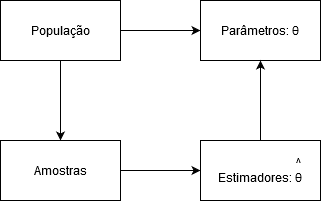
\includegraphics[width=0.5\linewidth]{diagrama}
	\caption{Esquema geral da Inferência.}
	\label{fig:diagrama}
\end{figure}

\pause
Estudaremos como se distribuem por amostragem o estimador $\bar{x}$ da média $\mu$, ou seja é uma estimativa para o parâmetro da população.

\end{frame}

\begin{frame}{Distribuição Amostral da Média}
	\textbf{Estimador da média $\mu$ populacional:} De uma população $X$ retiramos uma amostra de tamanho $n$ constituída pelos elementos $x_1,x_2,\dots,x_n$.
	
	\pause
	O estimador da média $\mu$ populacional da amostra é:
	$$\bar{x} = \displaystyle \frac{1}{n}\sum_{i=1}^{n}x_i$$
\end{frame}

\begin{frame}{Exemplo}
	Considere uma população finita $X$, onde:
	
	$$X:1,2,3,4,5$$
	
	\pause
	Logo, $N=5$.
	
	\pause
	Queremos mostrar que a esperança amostral $E(\bar{x})$ é igual a média $\mu$ populacional.
	
	\pause
	$E(x) = \mu_x = \displaystyle \sum_{i=1}^{N}x_i . p(x_i)$. \pause Dessa maneira, temos que:
	
	$$E(x) = \mu_x = \pause \displaystyle \frac{1+2+3+4+5}{5} = \pause \displaystyle \frac{15}{5} = \pause 3$$
	
	\pause
	
	Para a Variância usaremos: \pause $VAR(x) = \sigma_{x}^2 = \displaystyle \sum_{i=1}^{N}(x_i - \mu_x)^2 . p(x_i)$
\end{frame}

\begin{frame}{Exemplo}
	Criando uma Tabela:
	\centering
	\begin{tabular}{|c|c|c|c|c|}
		\hline 
		$x$ & $P(x)$ & $x - \mu_x$ & $(x - \mu_x)^2$ & $(x-\mu_x)^2 . P(x)$ \\ 
		\hline 
		1 & $\displaystyle \frac{1}{5}$ & -2 & 4 & $\displaystyle \frac{4}{5}$ \\ 
		\hline 
		2 & $\displaystyle \frac{1}{5}$ & -1 & 1 & $\displaystyle \frac{1}{5}$ \\ 
		\hline 
		3 & $\displaystyle \frac{1}{5}$ & 0 & 0 & 0 \\ 
		\hline 
		4 & $\displaystyle \frac{1}{5}$ & 1 & 1 & $\displaystyle \frac{1}{5}$ \\ 
		\hline 
		5 & $\displaystyle \frac{1}{5}$ & 2 & 4 & $\displaystyle \frac{4}{5}$ \\ 
		\hline 
		$\displaystyle \sum$ & 1 &  &  & 2 \\ 
		\hline 
	\end{tabular} 

\pause
Dessa maneira:
$$\sigma_{x}^2 = VAR(x) = 2$$
\end{frame}

\begin{frame}{Exemplo}
	Agora, seguindo nosso esquema inicial iremos retirar todas as amostras com reposição desta população finita. As amostras terão tamanho $n=2$. Assim, o número de amostras será: $N^n = 5^2 = 25$. Calcularemos a média amostral de todas as amostras.
	
	\pause
	\begin{center}
		
	\begin{tabular}{|c|c|c|}
		\hline 
		\multicolumn{2}{|c|}{Amostras} & $\bar{x}_i$ \\ 
		\hline 
		1 & (1,1) & 1,0 \\ 
		\hline 
		2 & (1,2) & 1,5 \\ 
		\hline 
		3 & (1,3) & 2,0 \\ 
		\hline 
		4 & (1,4) & 2,5 \\ 
		\hline 
		5 & (1,5) & 3,0 \\ 
		\hline 
		6 & (2,1) & 1,5 \\ 
		\hline 
		7 & (2,2) & 2,0 \\ 
		\hline 
		8 & (2,3) & 2,5 \\ 
		\hline 
		9 & (2,4) & 3,0 \\ 
		\hline 
		10 & (2,5) & 2,5 \\ 
		\hline 
	\end{tabular} 
\pause
\begin{tabular}{|c|c|c|}
	\hline 
	\multicolumn{2}{|c|}{Amostras} & $\bar{x}_i$ \\ 
	\hline 
	11 & (3,1) & 2,0 \\ 
	\hline 
	12 & (3,2) & 2,5 \\ 
	\hline 
	13 & (3,3) & 3,0 \\ 
	\hline 
	14 & (3,4) & 3,5 \\ 
	\hline 
	15 & (3,5) & 4,0 \\ 
	\hline 
	16 & (4,1) & 2,5 \\ 
	\hline 
	17 & (4,2) & 3,0 \\ 
	\hline 
	18 & (4,3) & 3,5 \\ 
	\hline 
	19 & (4,4) & 4,0 \\ 
	\hline 
	20 & (4,5) & 4,5 \\ 
	\hline 
\end{tabular} 
\pause
	\begin{tabular}{|c|c|c|}
		\hline 
		\multicolumn{2}{|c|}{Amostras} & $\bar{x}_i$ \\ 
		\hline 
		21 & (5,1) & 3,0 \\ 
		\hline 
		22 & (5,2) & 3,5 \\ 
		\hline 
		23 & (5,3) & 4,0 \\ 
		\hline 
		24 & (5,4) & 4,5 \\ 
		\hline 
		25 & (5,5) & 5,0 \\ 
		\hline 
		&  &  \\ 
		\hline 
		&  &  \\ 
		\hline 
		&  &  \\ 
		\hline 
		&  &  \\ 
		\hline 
		&  &  \\ 
		\hline 
	\end{tabular} 
	\end{center}
\end{frame}

\begin{frame}{Exemplo}
	Verificamos que $\bar{x}_i$ varia em cada uma das $25$ amostras, logo podemos analisar $\bar{x}_i$ como uma variável aleatória, neste caso, uma variável aleatória discreta. 
	\pause
	
	\begin{center}
	\begin{tiny}	
	\begin{tabular}{|c|c|c|c|}
		\hline 
		$\bar{x}$ & $P(\bar{x})$ & $\bar{x}.P(\bar{x})$ & $\bar{x}^2 . P(\bar{x})$ \\ 
		\hline 
		1,0 & $\displaystyle \frac{1}{25}$ & $\displaystyle \frac{1,0}{25}$ & $\displaystyle \frac{1}{25}$ \\ 
		\hline 
		1,5 & $\displaystyle \frac{2}{25}$ & $\displaystyle \frac{3,0}{25}$ & $\displaystyle \frac{4,5}{25}$ \\ 
		\hline 
		2,0 & $\displaystyle \frac{3}{25}$ & $\displaystyle \frac{6,0}{25}$ & $\displaystyle \frac{12}{25}$ \\ 
		\hline 
		2,5 & $\displaystyle \frac{4}{25}$ & $\displaystyle \frac{10,0}{25}$ & $\displaystyle \frac{25}{25}$ \\ 
		\hline 
		3,0 & $\displaystyle \frac{5}{25}$ & $\displaystyle \frac{15,0}{25}$ & $\displaystyle \frac{45}{25}$ \\ 
		\hline 
		3,5 & $\displaystyle \frac{4}{25}$ & $\displaystyle \frac{14}{25}$ & $\displaystyle \frac{49}{25}$ \\ 
		\hline 
		4,0 & $\displaystyle \frac{3}{25}$ & $\displaystyle \frac{12}{25}$ & $\displaystyle \frac{48}{25}$ \\ 
		\hline 
		4,5 & $\displaystyle \frac{2}{25}$ & $\displaystyle \frac{9}{25}$ & $\displaystyle \frac{40,5}{25}$ \\ 
		\hline 
		5,0 & $\displaystyle \frac{1}{25}$ & $\displaystyle \frac{5,0}{25}$ & $\displaystyle \frac{25}{25}$ \\ 
		\hline 
		$\displaystyle \sum$ & 1 & 3 & 10 \\ 
		\hline 
	\end{tabular} 
\end{tiny}
	\end{center}
\end{frame}

\begin{frame}{Exemplo}
	Dessa forma, utilizando a fórmula da Esperança, temos: \pause
	$$E(\bar{x}) = \mu_{\bar{x}} = \displaystyle \sum_{i=1}^{n}\bar{x}_i . P(\bar{x}_i) = 3$$ \pause
	O que resulta em:
	$$\mu_{\bar{x}} = E(\bar{x}) = 3$$
	
	\pause
	Como $E(\bar{x}^2) = \displaystyle \sum_{i=1}^{n}\bar{x}_i^2 . p(\bar{x}_i)$, resulta em: $E(\bar{x}^2) =10$
	
	\pause
	Vimos que uma outra forma de obter a variância é: 
	$$VAR(\bar{x}) = E(\bar{x}^2) - \{E(\bar{x})\}^2$$
	\pause
	Substituindo, segue:
	$$VAR(\bar{x}) = 10 - 3^2 = 1$$
	\pause
	Dessa forma:
	$$\sigma_{\bar{x}}^2 = VAR(\bar{x})=1$$
\end{frame}

\begin{frame}{Proposição 01}
	\textbf{Proposição 01:}	A média das médias amostras, ou $E(\bar{x})$, é igual à média $\mu$ populacional, ou $E(\bar{x}) = \mu_x$.
	
	\pause
	Quando temos $E(\hat{\theta}) = \theta$, o estimador $\hat{\theta}$ é não viciado, não viesado ou não tendencioso. Assim $\bar{x}$ é um estimador não tendencioso de $\mu$.
\end{frame}

\begin{frame}{Proposição 02}
	\textbf{Proposição 02:}	A variância da média amostral é igual à variância populacional dividida pelo tamanho da amostra, ou seja,
	$$VAR(\bar{x}) = \sigma_x^2 = \displaystyle \frac{\sigma^2}{n}$$
	
	\pause
	Ou seja, se $X:N(\mu,\sigma^2)$ e se dessa população retiramos amostras de tamanho $n$, então:
	$$\bar{x}:N\left( \mu, \displaystyle \frac{\sigma^2}{n} \right)$$
\end{frame}


\begin{frame}{Distribuição Amostral dos Estimadores}
	A distribuição da variável $\bar{x}$ por amostragem simples será sempre normal com a mesma média da população $X$ e a variância $n$ vezes menor. Ou seja, quanto maior a amostra menor a variância da média, ou seja, quanto maior a amostra maior a precisão do estimador $\bar{x}$.
	
	\pause
	{\bf O Fator de Correção} para populações finitas e de tamanho $N$ conhecido , e se a amostra de tamanho $n$ dela retirada for sem reposição, então:
	$$\sigma_{\bar{x}} = \displaystyle \frac{\sigma}{\sqrt{n}}\sqrt{\frac{N - n}{N - 1}}$$
\end{frame}

\begin{frame}{Exemplo 01}
	
	{\bf Exemplo 01:} Em uma população de $5000$ alunos de uma faculdade sabemos que a altura média dos alunos é $175$cm e o desvio padrão, $5$cm. Retiramos uma amostra sem reposição, de tamanho $n=100$. Determine o desvio padrão dessa amostra.
	
	
\end{frame}


\begin{frame}{Exemplo 01 - Solução}
	
	{\it Solução:}
	
	Temos que $X:N(175,25) \begin{cases}
	u = 175 \\
	\sigma = 5
	\end{cases}
	$
	
	\pause
	Então, $\sigma_{\bar{x}} = E(\bar{x}) = 175$
	
	\pause
	e
	$$\sigma_{\bar{x}} = \displaystyle \frac{\sigma}{\sqrt{n}}\sqrt{\frac{N - n}{N - 1}} = \displaystyle \frac{5}{10}\sqrt{\frac{5000 - 100}{5000 - 1}} = 0,495024$$
	
	\pause
	Assim, a média das médias amostrais é $175$cm e o desvio padrão da média amostral é $0,5$cm.
	
	
\end{frame}

\begin{frame}{Exemplo 01 - Solução}
	Se não utilizássemos o fator de correção, teríamos:
	\pause
	
	$$\sigma_{\bar{x}} = \displaystyle \frac{\sigma}{\sqrt{n}} = \frac{5}{10} = 0,5$$
	
	\pause
	Isto é, quando tiramos uma amostra grande de uma população muito maior que o da amostra (pelo menos o dobro), é indiferente usar o fator de correção para populações finitas, pois o erro é muito pequeno.
	
	\begin{flushright}
		$\blacksquare$
	\end{flushright}
\end{frame}

\begin{frame}{Dimensionamento de uma Amostra}
	Para determinarmos qual o tamanho da amostra que deveremos retirar para obter um erro de amostragem dentro de um risco determinado utilizamos o seguinte exemplo:
	
	\pause
	{\bf Exemplo 01:} Seja $X:N(1200,840)$. Qual deverá ser o tamanho da amostra de tal forma que $P(1.196 < \bar{x} <1204) = 0,9$?
	
	\pause
	{\it Solução:}
	
	Se $X:N(1200,840) \begin{cases}
	\mu = 1200 \\
	\sigma^2 = 840
	\end{cases}
	\therefore \sigma_{\bar{x}} = 1200
	$
	\pause
	e
	\pause
	$\sigma_{\bar{x}} = \displaystyle \frac{\sigma}{\sqrt{n}} = \frac{28,98}{\sqrt{n}} \therefore Z = \frac{\bar{x} - \mu}{\sigma_{\bar{x}}}$
	
	ou
	
	$Z_{\alpha} = Z_{0,45} = 1,64$
	
\end{frame}

\begin{frame}{Dimensionamento de uma Amostra}
	Assim,
	
	\pause
	$1,64 = \displaystyle \frac{1204 - 1200}{\frac{28,98}{\sqrt{n}}}$
	
	\pause
	É indiferente escolher o extremo inferior ou superior, sendo assim:
	
	$\displaystyle \sqrt{n} = \frac{1,64 \cdot 28,98}{4}$
	
	$\displaystyle \sqrt{n} = 11,88 \implies n = 141,13 \implies n \approx 141$
	
	\pause
	Com isso, concluímos que, se retirarmos uma amostra de $141$ elementos da população $X$, teremos $95\%$ de confiança que $\bar{x}$ estará no intervalo $(1.196,1.216)$, o que significa que o risco que corremos de que o valor da média caia fora do intervalo anterior é de $5\%$.
	\begin{flushright}
		$\blacksquare$
	\end{flushright}
\end{frame}


\end{document}

